
\subsection{1.20 Соединения переходных металлов 4 группы. Геометрия молекул в зависимости от природы лигандов, их электронное строение, способы получения и химическое поведение.}
\begin{itemize}
	\item $Ti$: $(+2), +3, +4$ \quad координационное число $6$ \quad $3d^24s^2$
	\item $Zr$: $(+2), +3, +4$ \quad координационные числа $7, 8$ \quad $4d^2 5s^2$
	\item $Hf$: $(+3), +4$ \quad координационные числа $7, 8$ \quad $4f^4 5d^2 6s^2$
\end{itemize}
\ul{Координационное число $6$}
\[
\left[TiF_6 \right]^{2-} \quad \left[Ti(H_2O)_6 \right]^{3+} \quad \left[TiCl_6 \right]^{3-} \quad \text{ октаэдр.}
\]
$d^1$, эффект Яна-Теллера:
\begin{figure} [H]
	\centering {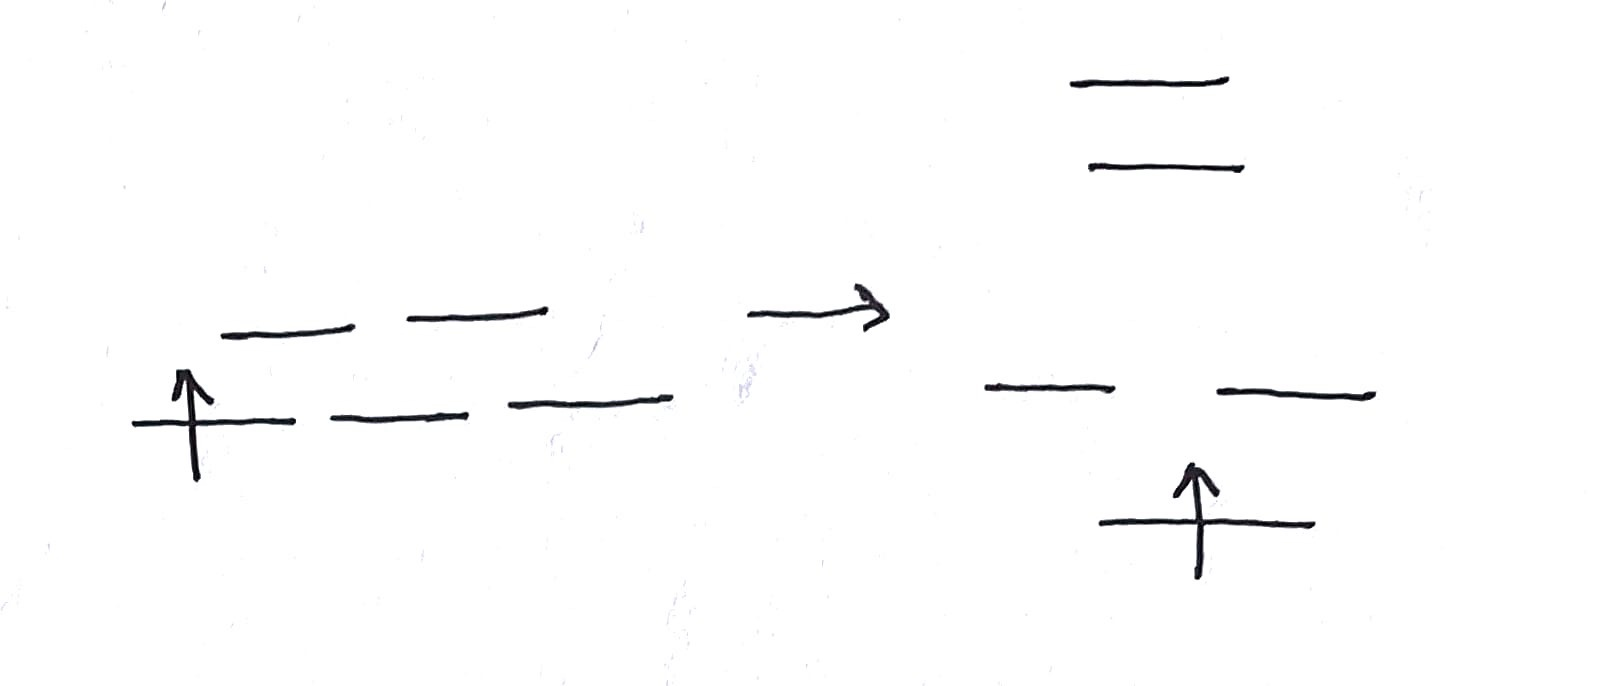
\includegraphics[scale=0.2]{aaq}}
\end{figure}
\textbf{Степень окисления $+3$} \\
$Ti^{+3}$ - восстановитель (с $KMnO_4, H_2O$) \\
$Ti$ в степени окисления $+4$ не образует устойчивых комплексов (ЭСКП $= 0$) \\
$ \left[ZrF_6 \right]^{2-} $ (КЧ = $6$)
\textbf{Степень окисления $+4$} \\
Соли титанила:
\begin{figure} [H]
	\centering {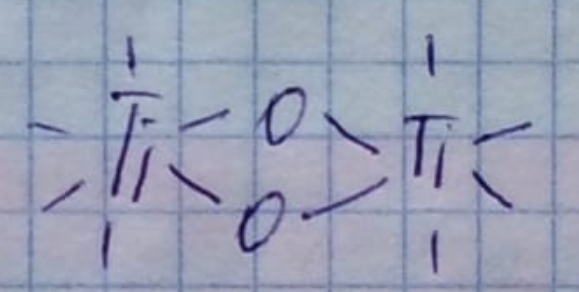
\includegraphics[scale=0.5]{aa1}}
\end{figure}
$d^0$ \\
\ul{Координационное число $7$}: $ \left[Zr^{+4}F_7 \right]^{3-} \quad \left[Hf^{+4}F_7 \right]^{3-} $ \\
\ul{Координационное число $8$}: $ \left[Zr^{+4}(ox)_4 \right]^{4-} \quad \left[Zr^{+4}(acac)_4 \right]^{4-} $ \\
\ul{Координационное число $4$}: $ \left[Hf(NPh_2)_4 \right] \quad \left[Zr(NPh_2)_4 \right] $ - стабилизируется объемными $L$ \\ \\
В природе:
\begin{itemize}
	\item рутил $TiO_2$
	\item циркон $ZrSiO_4$
	\item $Hf$ не образует собственных минералов
\end{itemize}
\begin{figure} [H]
	\centering {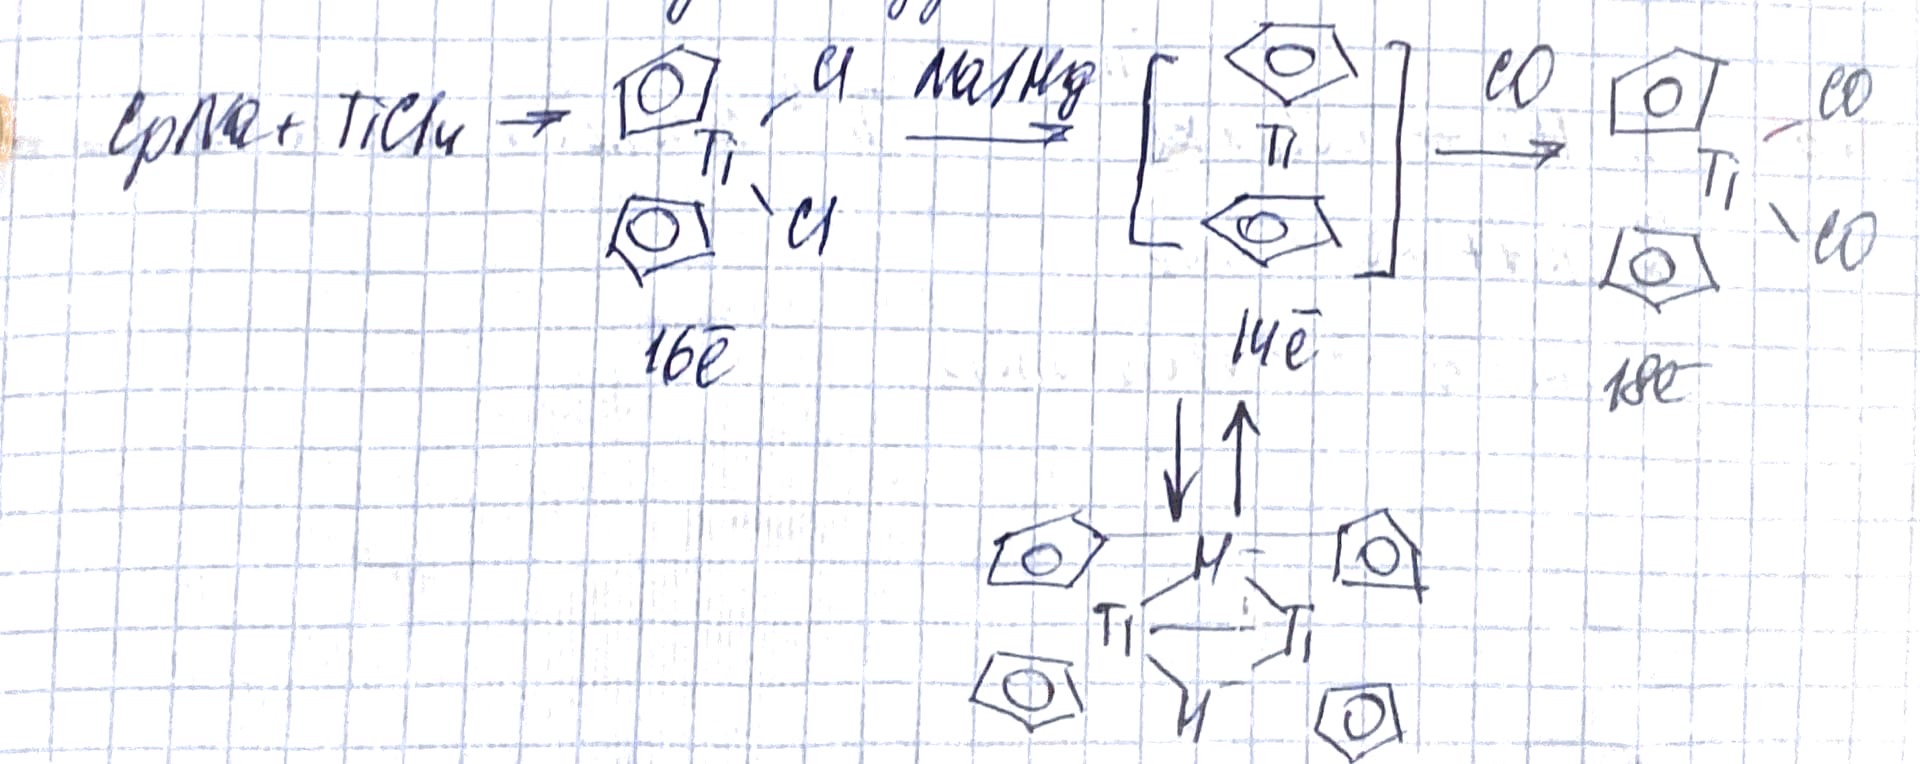
\includegraphics[scale=0.25]{aa2}}
\end{figure}
$Ti$: \\ 
\begin{itemize}
	\item Вскрытие руды
	\item $TiCl_4 + 2 Mg = Ti + 2MgCl_2$
	\item Очистка: $TiI_4 = Ti + 2I_2$
\end{itemize}
$Zr$: \\ 
\begin{itemize}
	\item Вскрытие минералов
	\item $ZrOSO_4 + 4 KF + 2HF = K_2\left[ZrF_6 \right] + H_2O + K_2SO_4$
	\item $K_2\left[ZrF_6 \right] + 4Na = Zr + 4NaF + 2KF$
	\item Очистка: $ZrI_4 = Zr + 2I_2$
\end{itemize}
Свойства:
\begin{itemize}
	\item $Ti$:
	\begin{itemize}
		\item $+ HCl = 2TiCl_3 + H_2$
		\item $+ KOH + H_2O = K_2TiO_3 + H_2 $
		\item $+ HF = H_2\left[TiF_6 \right] + H_2 $
		\item $+ Cl_2 = TiCl_4 $
		\item $+ HNO_3(\text{к}) = TiO_2 \cdot H_2O + NO_2 + H_2O $		
	\end{itemize}
	\item $Zr, Hf$:
	\begin{itemize}
		\item $+ HCl \not = $
		\item $+ KOH \not = $
		\item $+ HF \not = $
		\item $+ Cl_2 = ZrCl_2$
		\item $+ HNO_3(\text{к}) + HF  = H_2\left[ZrF_6 \right] + NO + H_2O $		
	\end{itemize}
\end{itemize}
\textbf{Степень окисления $+3$} 
\begin{align*}
Ti + HCl &= TiCl_3 + H_2 \quad \text{ $Ti^{+3}$ - сильный восстановитель, слабый окислителль}\\
ZrCl_4 + Zr &= ZrCl_3 \\
HfCl_4 + Al &= t = HfCl_3 + AlCl_3 
\end{align*}	
\textbf{Степень окисления $+4$} \\
Свойства: \\
$TiO_2$:
\begin{itemize}
	\item $+ C + Cl_2 = TiCl_4 + CO$
	\item $+ KOH = K_2TiO_3 + H_2 $
	\item $+ KH_2 = K_2TiF_6$
	\item $+ nH_2O = TiO(OH)_2 + H_2O	$	
\end{itemize}
Две формы существования титановой кислоты $TiO_2 \cdot 2H_2O$:
\begin{figure} [H]
	\centering {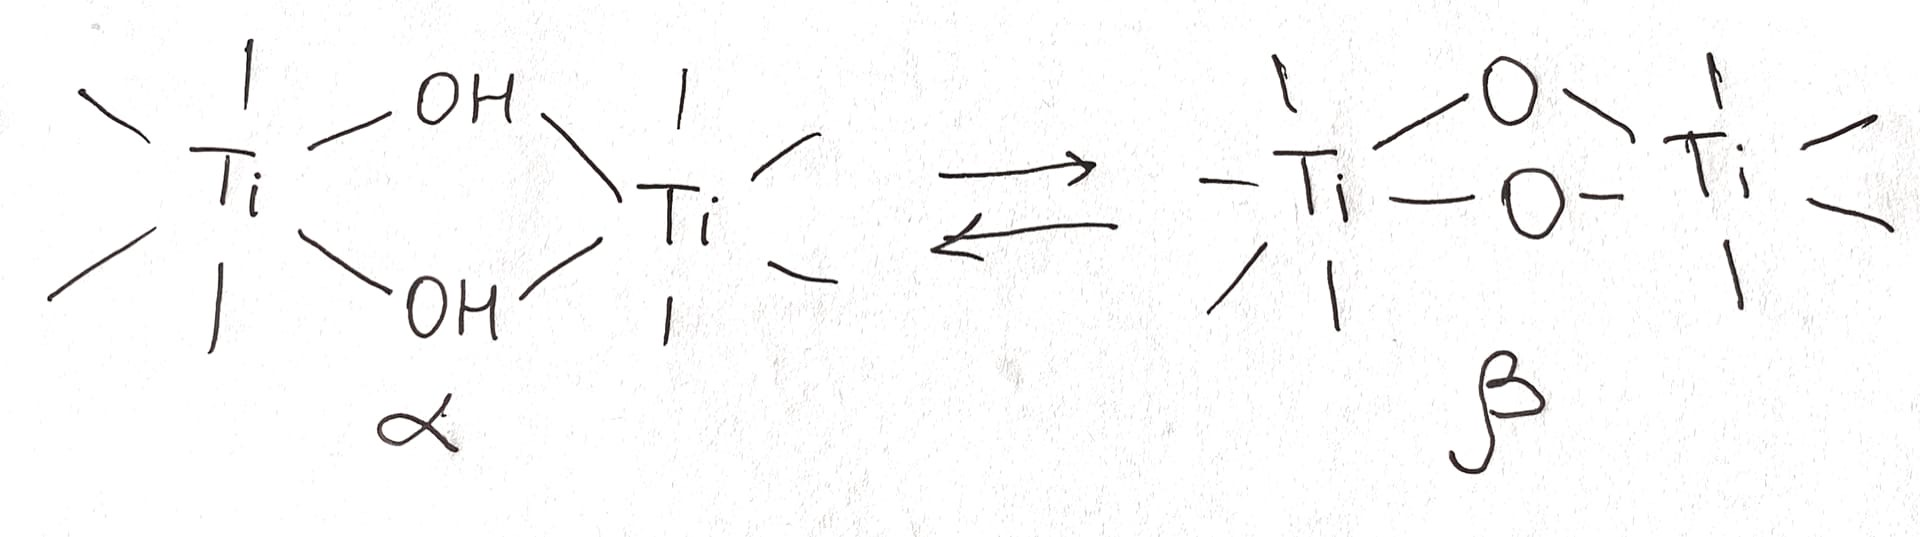
\includegraphics[scale=0.25]{aa3}}
\end{figure}
$TiCl_4$:
\begin{itemize}
	\item $+ H_2O + NaOH =TiO(OH)_2 $
	\item $+ H_2 = TiCl_3 + HCl$	
\end{itemize}
